%!TEX root = ../main.tex
\section{Method}
\subsection{Getting to know the data: Diagnostic plots of marginal return series}

\subsection{Univariate ARMA-GARCH modeling of factor return series}

\subsection{Rolling correlations}
We compute rolling correlation estimates in order to investigate whether the factor equity strategies exhibit constant correlation over time. 
\begin{align}
    RCorr(r_{i, t}, r_{j, t})_t^{w} = \frac{\sum^{t}_{t-w+1}(r_{i, t} - \bar{r}_i)(r_{j,t} - \bar{r}_j)}{\sqrt{\sum^{t}_{t-w+1} (r_{i,t} - \bar{r}_i)^2} \sqrt{\sum^{t}_{t-w+1} (r_{j,t} - \bar{r}_j)^2}}
\end{align}
where $r_i$, $r_j$ are the $N \cdot (N-1) / 2$ different pairs of the factor strategies' log returns and $w$ is the rolling window of data. We use approximately one year of data with $w = 45$ on weekly data.
\subsection{Threshold correlations}
Threshold (or exceedance) correlations have previously been used to highlight the tail dependence of i.a. country equity indices~\autocite{LonginSolnik2001}, portfolios by industry, size, value and momentum~\autocite{AngChen2002} and factor strategies~\autocite{ChristoffersenLanglois2013}. However, no paper has previously studied threshold correlation between factors when including the RMW and CMA factors. We follow~\textcite{ChristoffersenLanglois2013} definition of threshold correlation
\begin{align}
    TCorr(r_i, r_j) = 
    \begin{cases} 
        Corr\Big(r_i, r_j \,|\, r_i < F_i^{-1}(p), r_j < F_j^{-1}(p)\Big)  & \text{for } p < 0.5 \\
        Corr\Big(r_i, r_j \,|\, r_i \geq F_i^{-1}(p), r_j \geq F_j^{-1}(p)\Big)  & \text{for } p \geq 0.5
    \end{cases}
\end{align}
where $F_i^{-1}(p)$ the empirical quantile of $r_i$ at percentile $p$. Graphically, threshold correlation can be understood from \autoref{diag:thresholdexplain}. 
\begin{figure}[H]
  \caption{Threshold correlation - conceptual plot}
  \label{diag:thresholdexplain}
  %\toprule
  \centering
  \begin{minipage}{\textwidth}
  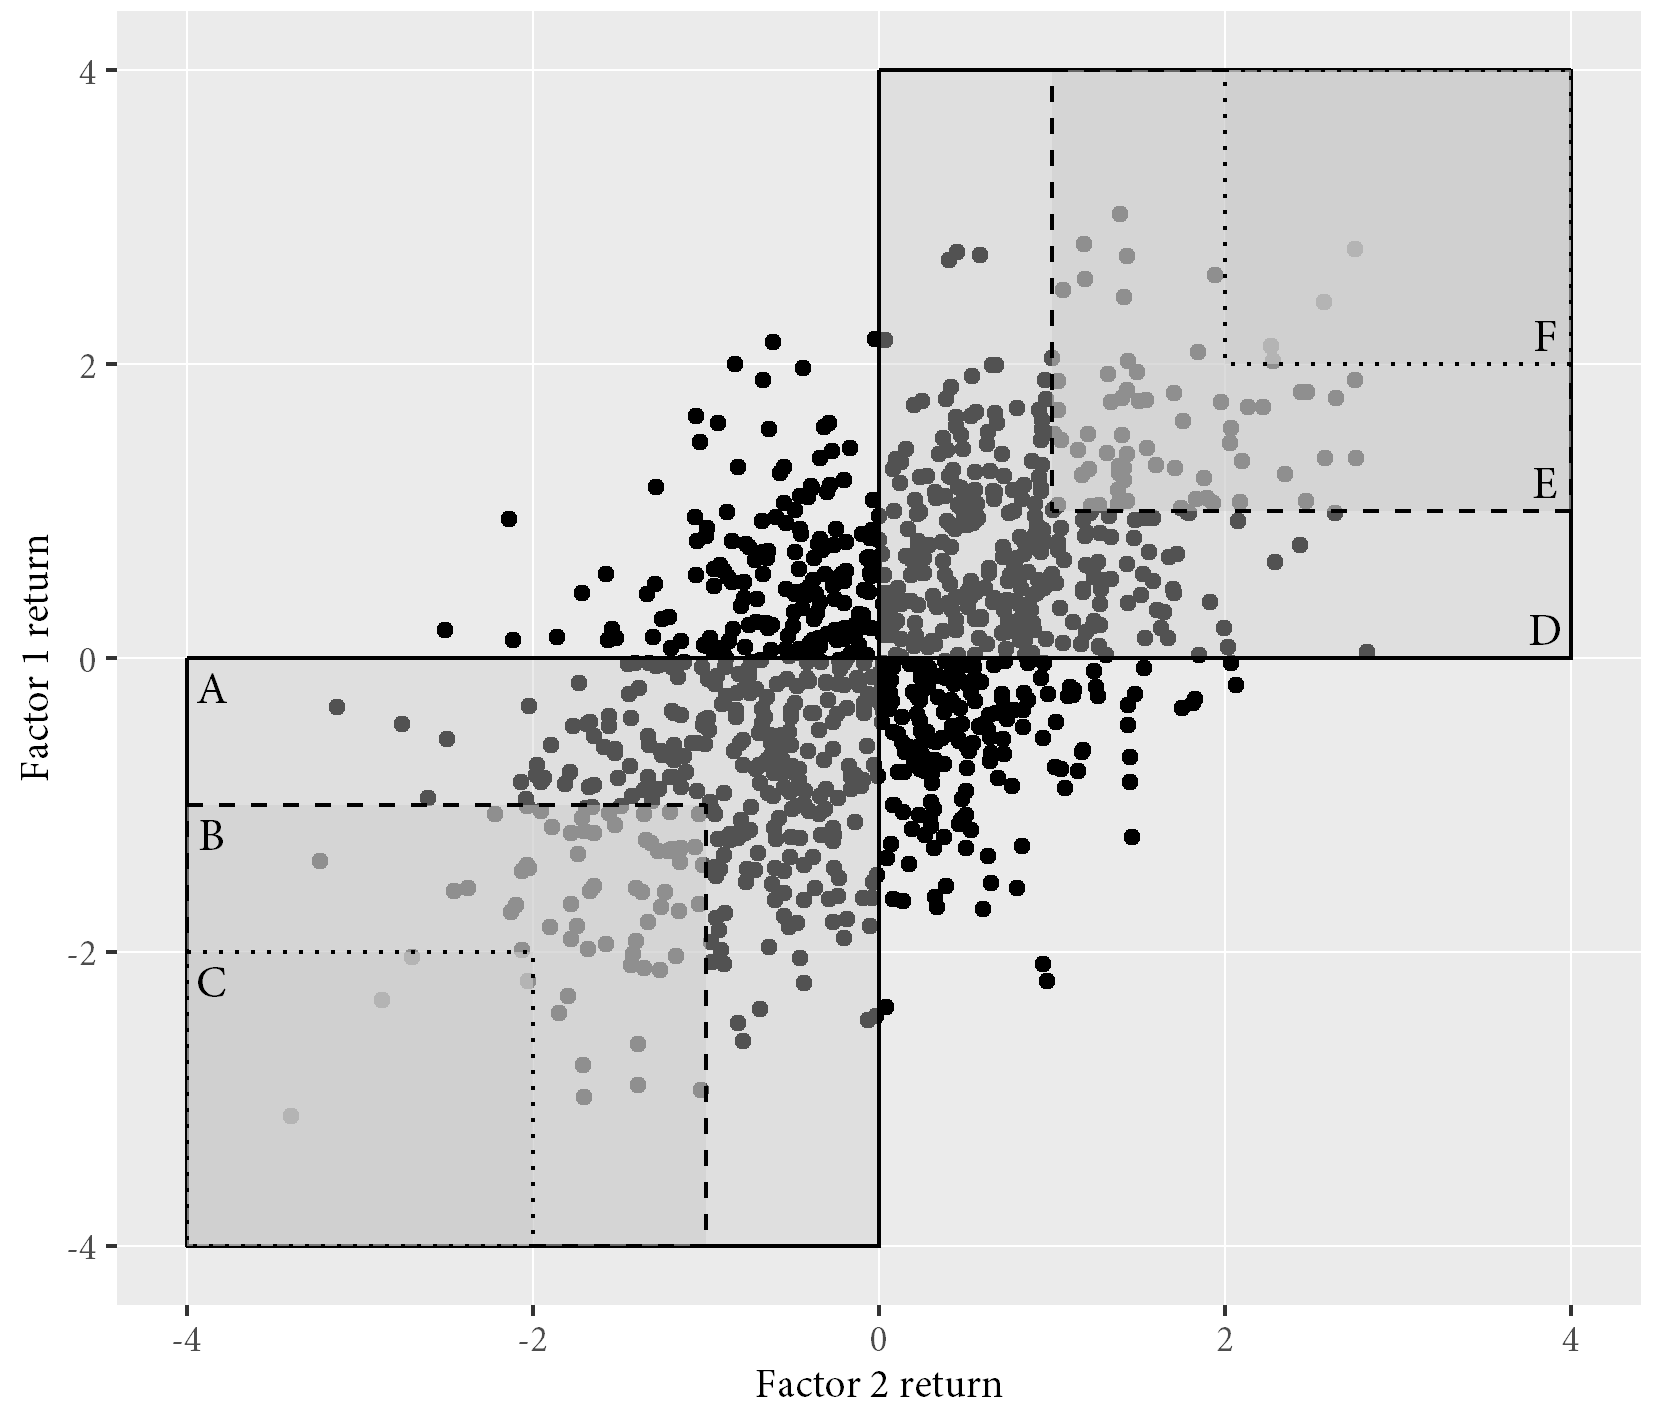
\includegraphics[scale=1]{graphics/threshold_explain.png}  
  %\bottomrule
  \vspace{3mm}
  \footnotesize
  Conceptual plot of threshold correlations coefficients. A, B and C areas represent threshold correlation subset of data when $p<0.50$ and D, E and F areas represent subsets when $p\geq0.50$. The data is a random generation of 1,000 observations from a bivariate standard normal distribution with correlation coefficient 0.5.
  \end{minipage}
\end{figure}
For $p = 0.49$, the first value below the median, threshold correlation is the linear correlation in the subset of data that is in area A. As $p$ approaches zero, the area A becomes smaller and smaller, illustrated by B and C. Above the median, the same is illustrated by areas D, E and F. Ceteris paribus, assets pairs with weaker or negative threshold correlation as $p < 0.50$ are better diversified, as they tend to coincide in extreme negative returns less often. Although threshold correlations are simply the linear correlations for a subset of the data, they do give a measure of tail dependency - how correlated are returns when times are extreme? Furthermore, they provide an indirect way of testing whether variables are jointly normal distributed, as the threshold correlation of normally distributed variables tends to zero as $p$ approaches zero or one. For jointly Student-\textit{t} distributed variables, this is not the case, and for jointly skewed Student-\textit{t} distributed variables, threshold correlations can also be asymmetric, i.e. different above and below the median.
\subsection{Copula}
Copulae provide a numerically feasible way to estimate a multivariate distribution function, which can then be used to draw inferences and simulate return series.~\textcite{Patton2006} uses the theorem of~\textcite{Sklar1959} to show that the conditional multivariate distribution function of log returns can be decomposed into a copula function and the product of univariate distributions
\begin{align} \label{eq:sklar}
    f_t(r_{1,t+1}, ..., r_{N, t+1}) &= c_t(u_{1, t+1}, ... u_{N, t+1}) \prod^N_{i=1} f_{i,t}(r_{i, t+1})
\end{align}
where $c_t(u_{1, t+1}, ... u_{N, t+1})$ is the copula density function, in this application taking uniform transformations of residuals from the ARMA-GARCH model, $\{u_i\}$, as arguments. This relies on a two-step maximum likelihood procedure (also known as the inference-by-margins (IFM) procedure) introduced by~\textcite{Joe1997}, which starts by estimating with the marginal distributions and subsequently estimates the copula function, using the margin residuals as given. For details on the marginal estimation procedure, see \autoref{App:AppendixB} The IFM method drastically improves the speed of the optimization process in large data sets; however, it is not efficient as shown by~\textcite{ChenFanTsyrennikov2006}, who instead propose a sieve ML estimation. This paper still employs IFM, as the efficiency loss is small in most cases~\autocite{Patton2006}. 

We focus on a skewed Student-\textit{t} copula, parameterized by $\Theta = \{\nu, \gamma, R\}$ using the constant correlation specification, and by $\Theta^{cDCC} = \{\nu, \gamma, \alpha, \beta, R\}$ using the dynamic correlation process. The analysis closely follows in the footsteps of~\textcite{Aielli2013} and~\textcite{ChristoffersenErrunzaJacobLanglois2012}. The skewed Student-\textit{t} distribution is described in detail in \autoref{App:AppendixA}.

The normal and Student-\textit{t} copulae are both nested in the skewed Student-\textit{t} model, as the degree of freedom and skewness parameters go to infinity and zero respectively. Results are presented for all three copulae, with and without correlation dynamics. The model selection criteria is BIC (\textcite{Schwarz1978}).

\textbf{Constant correlation specification}

As a benchmark model, we consider the case of a constant correlation matrix between the factor strategies' ARMA-GJR-GARCH residuals. 

The copula parameters $\Theta = \{\nu, \gamma, R_t\}$ are estimated using ML of the copula function, where $\nu$ is the degree of freedom, $\gamma$ is the vector of skewness parameters and $R$ is the constant copula correlation matrix. Rearranging Sklar's Theorem in \autoref{eq:sklar} and taking logs, the copula log-likelihood function is
\begin{align} \label{eq:constantllf}
    LLF(\nu, \gamma, R; u_1, ..., u_T) = \sum^T_{t=1} \Big \{ ln f_t(\varepsilon_{t}; \nu, \gamma, R) - \sum^N_{i = 1} ln f_{i,t}(\varepsilon_{i, t}; \nu, \gamma) \Big \}
\end{align}
where the density function $f$ is the skewed Student-\textit{t} given by \autoref{eq:dskewt}.

\textbf{\textit{c}DCC conditional correlation process}

To capture time-varying dependency, as motivated by rolling correlation and threshold correlation analyses, the copula correlation matrix $R_t$ is allowed to vary over time according to the \textit{c}DCC model~\autocite{Aielli2013}\footnote{\textit{c} stands for corrected, as Aielli (2009) has shown that the standard DCC estimator of Engle (2002) and Tse \& Tsui (2002) can be inconsistent.}
\begin{align} \label{eq:qtrtlink}
    R_t &= Q_t^{-1/2} Q_t Q_t^{-1/2}
    \intertext{where the core process is}
    Q_t &= (1 - \alpha - \beta) S + \alpha z_{t-1} z_{t-1}^\top + \beta Q_{t-1} \label{eq:qprocess}
\end{align}
The $Q_t$ process is comprised of three components that are weighted according to $\alpha, \beta$: (1) $S$, a time-invariant component, to be interpreted similarly to a long-term mean in a regular GARCH process as $\mathbb{E}[Q_t] = S$, (2) $z_{t-1} z_{t-1}^\top$, an innovation component from the copula shocks, and (3) $Q_{t-1}$, an autoregressive component of order one. In order for the the correlation matrix $R_t$ to be positive definite, $Q_t$ has to be positive definite, which is ascertained by requiring that $\alpha \geq 0$, $\beta \geq 0$ and $(\alpha + \beta) < 1$.

The parameters $\alpha, \beta$ are simultaneously estimated with the skewed Student-\textit{t} parameters $\nu$ and $\gamma$ using ML for the copula function, whose log-likelihood function is again found by rearranging Sklar's theorem (\autoref{eq:sklar}) and taking logs on both sides
\begin{align} \label{eq:cdccllf}
    LLF(\nu, \gamma, \alpha, \beta, R_t; u_1, ..., u_T) = \sum^T_{t=1} \Big \{ ln f_t(\varepsilon_{t}; \nu, \gamma, \alpha, \beta, R_t) - \sum^N_{i = 1} ln f_{i,t}(\varepsilon_{i, t}; \nu, \gamma) \Big \}
\end{align}
where the density function $f$ is the skewed Student-\textit{t} given by \autoref{eq:dskewt}.

The process of the copula estimation with \textit{c}DCC dynamics is quite involved, as it relies on moment matching and recursive estimation of parameters to estimate the copula correlation matrices $\{\hat{R_t}\}$. See \autoref{App:AppendixD} for a detailed description.

\textbf{Extending the cDCC model with exogenous regressors}

\Textcite{ChristoffersenErrunzaJacobLanglois2012} consider an extension of~\eqref{eq:qprocess}, where the long-running component $S$ is extended with a time-varying component in a general manner. Replace $S$ with a weighted average of a time-invariant component $\Omega$ and a time-varying component $\Upsilon_t$, to get:
\begin{align}
    S_t &= (1 - \phi) \Omega + \phi \Upsilon_t
\end{align}
$\Upsilon_t$ can support any number of common or factor-specific regressors, such as a common time-trend, conditional volatilities or arbitrage activity. We detail how we construct it in~\autoref{App:AppendixD}.

\begin{quote}
    \textit{Draft Note:} Using $\Upsilon_t$ we will be able to model how the dynamics of tail-dependency change with arbitrage activity, which relates to the second/extended parts of our paper. We have yet to get ahold of the data necessary to estimate this model. For practical purposes, we are looking to move forward with just one copula distribution (likely symmetric Student's t since the asymmetries don't appear that great).

    At its most simple, we can use a simple time trend as in~\autocite{ChristoffersenErrunzaJacobLanglois2012}. However, we would like to use data from Lipper, for which we don't have access yet.
\end{quote}

\textbf{Copula-based expected shortfall}

By simulating many runs of one-week-ahead copula shocks, we can find the simulated probability distributions for one-week-ahead factor strategy returns. The process is as follows
\begin{enumerate}[(i)]
    \item At $t = T$, generate 10,000 one-week-ahead random copula shock vectors $z_{T+1}$ according to the conditional copula correlation matrix $\hat{R}_{T+1}$
    \item Transform each $z_{T+1}$ vector to uniform shocks using copula parameters
    \item Transform each uniform shocks vector to GARCH residuals using marginal distribution parameters
    \item Forecast the ARMA-GJR-GARCH process using the residual vectors to get the simulated return vectors $r_{T+1}$
    \item Infer the empirical distribution function of $T+1$ returns using the simulated return vectors
    \item Repeat steps (i)-(v) at $t = T+1, T+2, ...$
\end{enumerate}
The VaR and ES are then found by
\begin{align}
    VaR_{i,T+1}^{1-\alpha} &= F_{i, T+1}^{-1}(\alpha | I^{sim}_T) \\
    ES_{i, T+1}^{1 - \alpha} &= E_t[r_{i,T+1} | r_{i,T+1} < VaR_{i,T+1}^{1-\alpha}]
\end{align}
where $F_{i, T+1}^{-1}(\alpha | I^{sim}_T)$ is the inverse empirical CDF (based on simulated data set $I^{sim}_t$) of asset $i$ at time $T+1$.

\subsection{Conditional diversification benefits}
As the copula has time-varying dependece, it must also have time-varying diversification benefits. We use a measure of conditional diversification benefits from \textcite{ChristoffersenErrunzaJacobLanglois2012} to determine how modern and classic value differ in terms of diversification benefits. 

The method is based on time-varying expected shortfall, expressed in percentage terms as
\begin{align}
    ES^p_{i,t}(r_{i,t}) = -\mathbb{E}_{t-1}[r_{i,t} | r_{i,t} \leq F_{i,t}^{-1}(p)]
\end{align}
where $r_{i,t}$ are simple returns of assets $i$ (to ensure that the weighted average return property of a portfolio holds) and $F_{i,t}^{-1}(p)$ is the conditional inverse CDF of returns for the $p\%$ quantile, which is also equivalent to the negative estimate of $p\%$ Value-at-Risk (VaR).

For the portfolio setting, return and expected shortfall are denoted as
\begin{align}
    R_{t} = \sum\limits^N_{i=1} w_{i,t} r_{i,t} \\
    ES^p_t(w_t) = -\mathbb{E}_{t-1}[R_{t} | R_{t} \leq F_{t}^{-1}(p)]
\end{align}
where $w_{i,t}$ are the dynamic portfolio weights and $F_{t}^{-1}(p)$ is the inverse CDF of the portfolio return $R$ at the $p\%$ quantile.

Unlike Value-at-Risk, expected shortfall is a coherent risk measure that is sub-additive across assets. Therefore, the combined risk measure of a portfolio is always smaller than or equal to the sum of the marginal risk measures.
\begin{align} \label{eq:es1}
    ES^p_t(w_t) \leq \sum\limits^N_{i=1} w_{i,t} ES^p_t(r_{i,t}) && \forall w_t \in \mathbb{R}
\end{align}
where $w_{i,t}$ are the dynamic portfolio weights. From the equality in \autoref{eq:es1}, we know that a upper bound on $ES$ is
\begin{align}
    \overline{ES}^p_t(w_t) = \sum\limits^N_{i=1} w_{i,t} ES^p_t(R_{i,t})
\end{align}
This corresponds to the case of zero diversification benefits. Similarly, a lower bound on the portfolio's $ES$ is
\begin{align}
    \underline{ES}^p_t(w_t) = -F^{-1}_t(w_t, p) 
\end{align}
where $F^-1_t(w_t, q)$ is the inverse CDF at time $t$ for the portfolio return with weights $w_t$. The lower bound is, in other words, equivalent to the case when the portfolio's $ES$ is equivalent to the portfolio's $VaR$.

The conditional diversification benefit statistic is now defined as
\begin{align}
    CDB_t(w_t,p) = \frac{\overline{ES}^p_t(w_t) - ES^p_t(w_t)}{\overline{ES}^p_t(w_t) - \underline{ES}^p_t(w_t)}
\end{align}

The intuition behind the statistic is best understood by focusing on the second term of the numerator and the denominator: when diversification benefits are high, the expected shortfall of a portfolio is relatively close to the Value-at-Risk, which makes the ratio close to one. When diversification benefits are poor, the expected shortfall is hardly different from the weighted average of individual expected shortfalls, and the ratio is close to zero.

The statistic is dependent on the calculation of $ES^p_t(w_t)$ which can only be found by simulation. In line with \textcite{ChristoffersenErrunzaJacobLanglois2012}, we maximize $CDB_t(w_t,p)$ at each time $t$ by simulating 10,000 draws of 1-week-ahead returns, using the skewed Student-\textit{t} copula model with \textit{c}DCC correlation dynamics. This yields a series of optimal $\{CDB^*\}$ for corresponding optimal dynamic weights $\{w^*_t\}$.

In the empirical results, we report three different graphs of $CDB^*$ when $p=5\%$, with different restrictions on portfolio weights in the optimization: In the first, three portfolios are available, one with all six factor strategies, one with classic value (all, but excluding RMW, CMA) and one with modern value (all, but excluding HML). In the second, two portfolios are available, one with all factors excluding HML, and one with all factors excluding CMA. This graph is meant to disentangle the risk of HML and CMA respectively. In the third, three portfolios are available, one with Mkt-RF, HML, SMB and Mom, one with Mkt-RF, SMB, Mom and CMA, and one with Mkt-RF, SMB, Mom and RMW. This graph is meant to look at the three value factors marginal contributions.

There are also two general restrictions on the portfolios: First, all factor weights must be positive, as the interpretation of a negative factor weight is the same as betting against the factor. Note that this does not mean that short sales are prohibited, as factor strategies are inherently long-short. Second, factor weights must sum to 1, as we do not consider the case of leverage.

\subsection{Mean-variance investing}
As the classic value factor is shown to add no alpha to a portfolio of the remaining four factors in the five-factor model \autocite{FF2015}, we examine the impact of excluding HML from the investible universe.

By simulating 10,000 draws of 1-week-ahead returns, using the skewed Student-\textit{t} copula model with \textit{c}DCC correlation dynamics, we can estimate the conditional expected return vector and variance-covariance matrix. This allows us to conduct mean-variance investing based on estimates from the copula model. As previously, we impose the two general restrictions that all factor weights must be positive, and that factor weights must sum to 1, which makes the tangency portfolio without a risk-free asset the optimal portfolio. At the end of each week $t$, the optimization problem becomes
\begin{align}
    \max_{w} w^\top \mu - \frac{\gamma}{2}\,w^\top \Sigma w && s.t. w^\top \mathbf{1}_N = 1
\end{align}
where $w$ is the set of weights, $\mu$ is the expected return, $\gamma$ is the risk aversion, $\Sigma$ is the variance-covariance matrix, and $\mathbf{1}_N$ is a vector of ones. The tangency portfolio solution is
\begin{align}
    w^* = \frac{1}{\mu^\top \Sigma^{-1} \mathbf{1}_N} \, \Sigma^{-1} \mu
\end{align}
In parallel, we consider two investible asset universes, one with all six factor strategies and one without HML. We then consider the impact of excluding HML on a number of realized performance measures including: Sharpe ratio, maximum drawdown and skewness. [The hypothesis is that there will only be a minor impact on the Sharpe ratio, while maximum drawdown and skewness improve]
